\section{Results: Do Attribution Graphs Preserve Depth?}
\begin{table}[t]\centering\caption{Replacement fidelity at a matched budget (128 features/layer, TopK $k=8$, identical training).}\label{tab:fid}\scriptsize\begin{tabular}{rlrrrrr}\toprule
$D$ & replacement & $k$ & features/layer & params & rel. MSE & e2e acc\\\midrule
1 & CLT & 4 & 128 & 16576 & 0.0017 & 1.000\\
1 & CLT & 8 & 128 & 16576 & 0.0011 & 1.000\\
1 & CLT & 16 & 128 & 16576 & 0.0007 & 1.000\\
1 & PLT & 4 & 128 & 16576 & 0.0016 & 1.000\\
1 & PLT & 8 & 128 & 16576 & 0.0011 & 1.000\\
1 & PLT & 16 & 128 & 16576 & 0.0007 & 1.000\\
1 & PLTpm & 4 & 128 & 16576 & 0.0017 & 1.000\\
1 & PLTpm & 8 & 128 & 16576 & 0.0011 & 1.000\\
1 & PLTpm & 16 & 128 & 16576 & 0.0007 & 1.000\\
2 & CLT & 4 & 128 & 41344 & 0.0025 & 1.000\\
2 & CLT & 8 & 128 & 41344 & 0.0017 & 1.000\\
2 & CLT & 16 & 128 & 41344 & 0.0013 & 1.000\\
2 & PLT & 4 & 128 & 33152 & 0.0024 & 1.000\\
2 & PLT & 8 & 128 & 33152 & 0.0018 & 1.000\\
2 & PLT & 16 & 128 & 33152 & 0.0013 & 1.000\\
2 & PLTpm & 4 & 160 & 41408 & 0.0025 & 1.000\\
2 & PLTpm & 8 & 160 & 41408 & 0.0017 & 1.000\\
2 & PLTpm & 16 & 160 & 41408 & 0.0012 & 1.000\\
3 & CLT & 4 & 128 & 74304 & 0.0015 & 1.000\\
3 & CLT & 8 & 128 & 74304 & 0.0012 & 1.000\\
3 & CLT & 16 & 128 & 74304 & 0.0010 & 1.000\\
3 & PLT & 4 & 128 & 49728 & 0.0020 & 1.000\\
3 & PLT & 8 & 128 & 49728 & 0.0015 & 1.000\\
3 & PLT & 16 & 128 & 49728 & 0.0011 & 1.000\\
3 & PLTpm & 4 & 192 & 74496 & 0.0020 & 1.000\\
3 & PLTpm & 8 & 192 & 74496 & 0.0013 & 1.000\\
3 & PLTpm & 16 & 192 & 74496 & 0.0010 & 1.000\\
4 & CLT & 4 & 128 & 115456 & 0.0015 & 1.000\\
4 & CLT & 8 & 128 & 115456 & 0.0009 & 1.000\\
4 & CLT & 16 & 128 & 115456 & 0.0007 & 1.000\\
4 & PLT & 4 & 128 & 66304 & 0.0030 & 1.000\\
4 & PLT & 8 & 128 & 66304 & 0.0013 & 1.000\\
4 & PLT & 16 & 128 & 66304 & 0.0010 & 1.000\\
4 & PLTpm & 4 & 223 & 115324 & 0.0028 & 1.000\\
4 & PLTpm & 8 & 223 & 115324 & 0.0011 & 1.000\\
4 & PLTpm & 16 & 223 & 115324 & 0.0008 & 1.000\\
\bottomrule\end{tabular}
\end{table}
\begin{table}[t]\centering\caption{Effective graph depth (signed, root inputs) at $k=8$; 95\% bootstrap CI over certified seeds.}\label{tab:depth}\scriptsize\begin{tabular}{rlrrrrr}\toprule
$D$ & repl. & seeds & $D_\mathrm{feat}$ [95\% CI] & DCR & skip mass & direct frac.\\\midrule
1 & CLT & 5 & 1.00 [1.00, 1.00] & 1.00 & 0.00 & 0.14\\
1 & PLT & 5 & 1.00 [1.00, 1.00] & 1.00 & 0.00 & 0.14\\
1 & PLTpm & 5 & 1.00 [1.00, 1.00] & 1.00 & 0.00 & 0.14\\
2 & CLT & 5 & 1.50 [1.43, 1.58] & 0.75 & 0.19 & 0.12\\
2 & PLT & 5 & 1.46 [1.39, 1.52] & 0.73 & 0.14 & 0.12\\
2 & PLTpm & 5 & 1.43 [1.37, 1.49] & 0.71 & 0.14 & 0.11\\
3 & CLT & 4 & 1.93 [1.89, 1.97] & 0.64 & 0.38 & 0.04\\
3 & PLT & 4 & 1.97 [1.93, 2.01] & 0.66 & 0.27 & 0.04\\
3 & PLTpm & 4 & 1.94 [1.87, 2.00] & 0.65 & 0.27 & 0.05\\
4 & CLT & 1 & 2.03 [2.03, 2.03] & 0.51 & 0.48 & 0.05\\
4 & PLT & 1 & 2.01 [2.01, 2.01] & 0.50 & 0.33 & 0.05\\
4 & PLTpm & 1 & 2.00 [2.00, 2.00] & 0.50 & 0.31 & 0.05\\
\bottomrule\end{tabular}
\end{table}
\begin{figure}[t]\centering
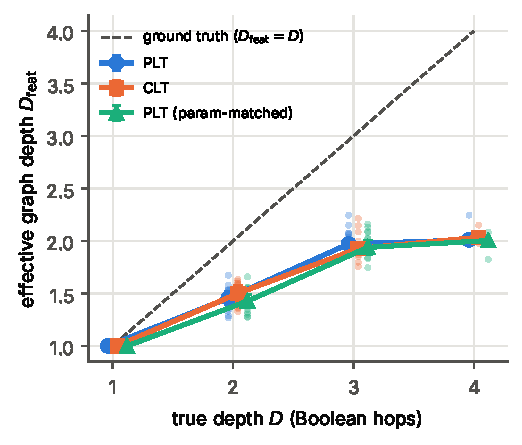
\includegraphics[width=0.45\linewidth]{figures/fig1_depth_vs_D.pdf}\\[4pt]
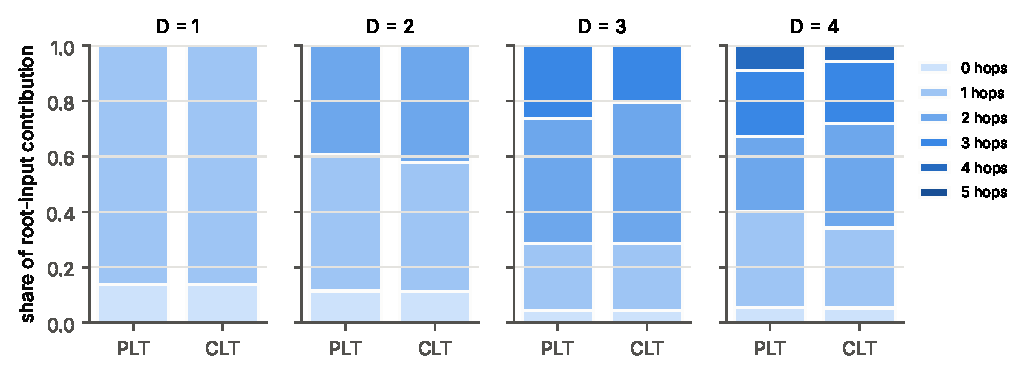
\includegraphics[width=0.95\linewidth]{figures/fig2_hop_profile.pdf}
\caption{Top: $\Dfeat$ vs.\ certified depth (dashed line: ground truth). Bottom: share of the root-input contribution by number of feature hops.}\label{fig:depth}\end{figure}
\paragraph{Both replacements reconstruct almost perfectly.} At the same budget, every replacement reaches relative MSE $\le\RelMSEMax$, and the full replacement model scores at least $\EtoEAccMin$ bit accuracy (Table~\ref{tab:fid}).
\paragraph{Both lose depth.} Graph depth grows with true depth, but much more slowly. At $D=3$, $\Dfeat=\DfeatCLTDThree$ for the CLT and $\DfeatPLTDThree$ for the PLT (DCR $\DCRCLTDThree$ and $\DCRPLTDThree$). At $D=4$ the DCR falls to $\DCRCLTDFour$ and $\DCRPLTDFour$ (Table~\ref{tab:depth}, Fig.~\ref{fig:depth}). Depth loss increases with $D$ for both replacement types (Spearman $\rho=\TrendRhoCLT$ for CLT, $\TrendRhoPLT$ for PLT).
\paragraph{At a matched budget, the headline depth gap is small.} The paired CLT$-$PLT difference in $\Dfeat$ is $\DiffCLTPLTDTwo$, $\DiffCLTPLTDThree$ and $\DiffCLTPLTDFour$ at $D=2,3,4$, with sign-flip $p=\PvalDTwo$, $\PvalDThree$ and $\PvalDFour$. The CLT does place more mass on edges that skip layers: $\SkipCLTDThree$ vs.\ $\SkipPLTDThree$ at $D=3$, and $\SkipCLTDFour$ vs.\ $\SkipPLTDFour$ at $D=4$.
% PILOT (3 seeds). Re-state after the full 5-seed run, the k-sweep and the param-matched PLT.
